\chapter{INSIDE {\iqist}}
\section{Basic theory and methods}

In this section, we will present the basic principles of CT-QMC impurity solvers, with an emphasis on the hybridization expansion technique. For detailed derivations and explanations, please refer to Ref.~\cite{RevModPhys.83.349}.

\subsection{Quantum impurity model}

The multi-orbital Anderson impurity model (AIM) can be written as $H_{\text{imp}} = H_{\text{loc}} + H_{\text{bath}} + H_{\text{hyb}}$, where
\begin{subequations}
\label{eq:aimp}
\begin{align}
& H_{\text{loc}} = \sum_{\alpha\beta} E_{\alpha\beta} d_{\alpha}^{\dagger} d_{\beta}+\sum_{\alpha\beta\gamma\delta} U_{\alpha\beta\gamma\delta} 
    d^{\dagger}_{\alpha}d^{\dagger}_{\beta} d_{\gamma} d_{\delta}, \\
& H_{\text{hyb} } = \sum_{\textbf{k}\alpha\beta} V^{\alpha\beta}_{\textbf{k}} c_{\textbf{k}\alpha}^{\dagger} d_{\beta} + h.c., \\
& H_{\text{bath}} = \sum_{\textbf{k}\alpha} \epsilon_{\textbf{k}\alpha} c_{\textbf{k}\alpha}^{\dagger} c_{\textbf{k}\alpha}.
\end{align}
\end{subequations}
In Eq.~(\ref{eq:aimp}), Greek letters in the subscripts denote a combined spin-orbital index, the operator $d_\alpha^{\dagger}$ ($d_\alpha$) is creating (annihilating) an electron with index $\alpha$ on the impurity site, while $c_{\textbf{k}\alpha}^{\dagger}$ ($c_{\textbf{k}\alpha}$) is the creation (annihilation) operator for conduction band (bath) electron with spin-orbital index $\alpha$ and momentum $\textbf{k}$. The first term in $H_{\text{loc}}$ is the general form of the impurity single particle term with level splitting and inter-orbital hybridization. This term can be generated by crystal field (CF) splitting or spin-orbit coupling (SOC), etc. The second term in $H_{\text{loc}}$ is the Coulomb interaction term which can be parameterized by intra(inter)-band Coulomb interactions $U$ $(U')$ and Hund's rule coupling $J$ or Slater integral parameters $F^{k}$. The hybridization term $H_{\text{hyb}}$ describes the process of electrons hopping from the impurity site to the environment and back. $H_{\text{bath}}$ describes the non-interacting bath. This Anderson impurity model is solved self-consistently in the DMFT calculations.

\subsection{Principles of continuous-time quantum Monte Carlo algorithm}

We first split the full Hamiltonian $H_{\text{imp}}$ into two separate parts, $H_{\text{imp}} = H_1 + H_2$, then treat $H_2$ as a perturbation term, and expand the partition function $\mathcal{Z} = \text{Tr} e^{-\beta H}$ in powers of $H_2$,
\begin{equation}
\label{eq:partition}
\mathcal{Z} = \sum_{n=0}^{\infty} \int_{0}^{\beta} \cdots \int_{\tau_{n-1}}^\beta \omega(\mathcal{C}_n),
\end{equation}
with
\begin{equation}
\label{eq:weight}
\omega(\mathcal{C}_n)=d\tau_1 \cdots d\tau_n \text{Tr}\left\{ e^{-\beta H_1}[-H_2(\tau_n)]\cdots [-H_2(\tau_1)]\right\},
\end{equation}
where $H_2(\tau)$ is defined in the interaction picture with $H_2(\tau) = e^{\tau H_1} H_2 e^{-\tau H_1}$. Each term in Eq.~(\ref{eq:partition}) can be regarded as a diagram or configuration (labelled by $\mathcal{C}$), and $\omega(\mathcal{C}_n)$ is the diagrammatic weight of a specific order-$n$ configuration. Next we use a stochastic Monte Carlo algorithm to sample the terms of this series. In the CT-INT and CT-AUX impurity solvers~\cite{PhysRevB.72.035122,Gull2008}, the interaction term is the perturbation term, namely, $H_2 = H_{\text{int}}$, while $H_2 = H_{\text{hyb}}$ is chosen for the CT-HYB impurity solver~\cite{PhysRevLett.97.076405}. In the intermediate and strong interaction region, CT-HYB is much more efficient than CT-INT and CT-AUX. This is also the main reason that we only implemented the CT-HYB impurity solvers in the $i$QIST software package.

\subsection{Hybridization expansion}

In the hybridization expansion algorithm, due to fact that $H_1$ does not mix the impurity and bath states, 
the trace in Eq.~(\ref{eq:weight}) can be written as $\text{Tr} = \text{Tr}_d \text{Tr}_c$. 
As a result, we can split the weight of each configuration as 
\begin{equation}
\omega(\mathcal{C}_n) = \omega_{d}(\mathcal{C}_n) \omega_{c}(\mathcal{C}_n) \prod\limits_{i=1}^{n} d\tau_i.
\end{equation}
$\omega_{d}(\mathcal{C}_n)$ is the trace over impurity operators ($\text{Tr}_d$), $\omega_{c}(\mathcal{C}_n)$ is the trace over bath operators ($\text{Tr}_c$). Further, since the Wick's theorem is applicable for the $\omega_c(\mathcal{C}_n)$ part, we can represent it as a determinant of a matrix $\mathcal{Z}_{\text{bath}}\mathcal{M}^{-1}$ with $\mathcal{Z}_{\text{bath}}=\text{Tr}_c e^{-\beta H_{\text{bath}}}$ and $(\mathcal{M}^{-1})_{ij} = \Delta(\tau_i - \tau_j)$. The $\omega_{d}(\mathcal{C}_n)$ part can be expressed using segment representation when $[n_{\alpha}, H_{\text{loc}}] = 0$~\cite{PhysRevLett.97.076405}. However, if this condition is not fulfilled, we have to calculate the trace explicitly, which is called the general matrix algorithm~\cite{PhysRevB.75.155113,PhysRevB.74.155107}. The explicit calculation of the trace for a large multi-orbital AIM with general interactions is computationally expensive. Many tricks and strategies have been implemented in the $i$QIST software package to address this challenge. Please refer to Sec.~\ref{sec:implement} for more details.

In this package, we used importance sampling and the Metropolis algorithm to evaluate Eq.~(\ref{eq:partition}). 
The following four local update procedures, with which the ergodicity of Monte Carlo algorithm is guaranteed, are used to generate the Markov chain: 
\begin{itemize}
\item Insert a pair of creation and annihilation operators in the time interval $[0,\beta)$.
\item Remove a pair of creation and annihilation operators from the current configuration.
\item Select a creation operator randomly and shift its position on the imaginary time axis.
\item Select a annihilation operator randomly and shift its position on the imaginary time axis.
\end{itemize}
In the Monte Carlo simulations, sometimes the system can be trapped by some (for example symmetry-broken) state. In order to avoid unphysical trapping, we also consider the following two global updates:
\begin{itemize}
\item Swap the operators of randomly selected spin up and spin down flavors.
\item Swap the creation and annihilation operators globally.
\end{itemize}

\subsection{Physical observables}

Many physical observables are measured in our CT-HYB impurity solvers. Here we provide a list of them.

\underline{Single-particle Green's function $G(\tau)$}

The most important observable is the single-particle Green's function $G(\tau)$, which is measured using the elements of the matrix $\mathcal{M}$, 
\begin{align}
\label{eq:gt}
G(\tau) = \left\langle \frac{1}{\beta} \sum_{ij}\delta^{-}(\tau, \tau_i - \tau_j) \mathcal{M}_{ji}\right\rangle,
\end{align}
with 
\begin{align}
\delta^{-}(\tau, \tau') = 
\begin{cases} 
\delta(\tau - \tau'), & \tau' > 0, \\
-\delta(\tau - \tau' + \beta), & \tau' < 0.
\end{cases}
\end{align}
Note that in the $i$QIST software package, the Matsubara Green's function $G(i\omega_n)$ is also measured directly, instead of being calculated from $G(\tau)$ using Fourier transformation.

\underline{Two-particle correlation function $\chi_{\alpha\beta}(\tau_a,\tau_b,\tau_c,\tau_d)$}

The two-particle correlation functions are often used to construct lattice susceptibilities within DMFT and diagrammatic extensions of DMFT. However, the measurements of two-particle correlation functions are a nontrivial task~\cite{PhysRevB.83.085102} as it is very time-consuming to obtain good quality data, and most of the previous publications in this field are restricted to measurements of two-particle correlation functions in one-band models. Thanks to the development of efficient CT-HYB algorithms, the calculation of two-particle correlation functions for multi-orbital impurity models now become affordable~\cite{PhysRevB.84.075145,PhysRevB.89.235128,PhysRevB.85.205106}. In the $i$QIST software package, we implemented the measurement for the two-particle correlation function $\chi_{\alpha\beta}(\tau_a,\tau_b,\tau_c,\tau_d)$, which is defined as follows:
\begin{equation}
\chi_{\alpha\beta}(\tau_a,\tau_b,\tau_c,\tau_d)
= \langle c_{\alpha}(\tau_a)c^{\dagger}_{\alpha}(\tau_b)c_{\beta}(\tau_c)c^{\dagger}_{\beta}(\tau_d)\rangle.
\end{equation}
Due to the memory restrictions, the actual measurement is performed in the frequency space, for which we use the following definition of the Fourier transform:
\begin{align}
\chi_{\alpha\beta}(\omega,\omega',\nu) &= \frac{1}{\beta}
\int^{\beta}_{0}d\tau_a\int^{\beta}_{0}d\tau_b\int^{\beta}_{0}d\tau_c\int^{\beta}_{0}d\tau_d
\nonumber\\
&\times \chi_{\alpha\beta}(\tau_a,\tau_b,\tau_c,\tau_d) 
e^{i(\omega+\nu)\tau_a}e^{-i\omega\tau_b}e^{-i\omega'\tau_c}e^{-i(\omega'+\nu)\tau_d}.
\end{align}
where $\omega$ and $\omega'$ [$\equiv (2n+1)\pi\beta$] are fermionic frequencies, and $\nu$ is bosonic ($\equiv 2n\pi/\beta$).

\underline{Local irreducible vertex functions $\Gamma_{\alpha\beta}(\omega,\omega',\nu)$}

From the two-particle Green's function $\chi_{\alpha\beta}(\omega,\omega',\nu)$, the local irreducible vertex function $\Gamma_{\alpha\beta}(\omega,\omega',\nu)$ can be calculated easily, via the Bethe-Salpeter equation~\cite{PhysRevB.86.125114,PhysRevB.85.205106,PhysRevB.89.235128}:
\begin{equation}
\Gamma_{\alpha\beta}(\omega,\omega',\nu) = 
\frac{\chi_{\alpha\beta}(\omega,\omega',\nu) 
- \beta[G_\alpha(\omega+\nu)G_\beta(\omega')\delta_{\nu,0} 
- G_\alpha(\omega+\nu) G_\beta(\omega') \delta_{\alpha\beta}\delta_{\omega\omega'}]}
{G_\alpha(\omega+\nu)G_\alpha(\omega)G_\beta(\omega')G_\beta(\omega'+\nu)}.
\end{equation}
The $G(i\omega_n)$ and $\Gamma_{\alpha\beta}(\omega,\omega',\nu)$ are essential inputs for the Parquet post-processing code, see Sec.~\ref{subsec:parquet} for more details.

\underline{Impurity self-energy function $\Sigma(i\omega_n)$}

The self-energy $\Sigma(i\omega_n)$ is calculated using Dyson's equation directly
\begin{equation}
\Sigma(i\omega_n) = G^{-1}_{0}(i\omega_n) - G^{-1}(i\omega_n),
\end{equation}
 or measured using the so-called improved estimator~\cite{PhysRevB.89.235128,PhysRevB.85.205106}. Noted that now the latter approach only works when the segment representation is used. Please check Sec.~\ref{subsec:self} for more details.

\underline{Histogram of the perturbation expansion order}

We record the histogram of the perturbation expansion order $k$, which can be used to evaluate the kinetic energy [see Eq.~(\ref{eq:kin})].

\underline{Occupation number and double occupation number}

The orbital occupation number $\langle n_\alpha\rangle$ and double occupation number $\langle n_\alpha n_\beta \rangle$ are measured. From them we can calculate for example the charge fluctuation $\sqrt{\langle N^2 \rangle - \langle N \rangle^2}$, where $N$ is the total occupation number:
\begin{equation}
N = \sum_{\alpha} n_{\alpha}.
\end{equation}

\underline{Spin-spin correlation function}

For a system with spin rotational symmetry, the expression for the spin-spin correlation function reads 
\begin{equation}
\chi_{ss}(\tau) = \langle S_{z}(\tau) S_{z}(0) \rangle,
\end{equation}
where $S_{z} = n_{\uparrow} - n_{\downarrow}$. From it we can calculate the effective magnetic moment:
\begin{equation}
\mu_{\text{eff}} = \int^{\beta}_{0}d\tau \chi_{ss}(\tau).
\end{equation}

\underline{Orbital-orbital correlation function}

The expression for the orbital-orbital correlation function reads 
\begin{equation}
\chi^{nn}_{\alpha\beta}(\tau) = \langle n_{\alpha}(\tau) n_{\beta}(0) \rangle.
\end{equation}

\underline{Kinetic energy}

The expression for the system kinetic energy reads
\begin{equation}
\label{eq:kin}
E_\text{kin} = -\frac{1}{\beta} \langle k \rangle,
\end{equation}
where $k$ is the perturbation expansion order.

\underline{Atomic state probability}

The expression for the atomic state probability is 
\begin{equation}
p_{\Gamma} = \langle |\Gamma \rangle \langle \Gamma| \rangle,
\end{equation}
where $\Gamma$ is the atomic state.

\subsection{Two-particle measurements and DMFT + Parquet formalism\label{subsec:parquet}}

\begin{figure}[tp]
\centering
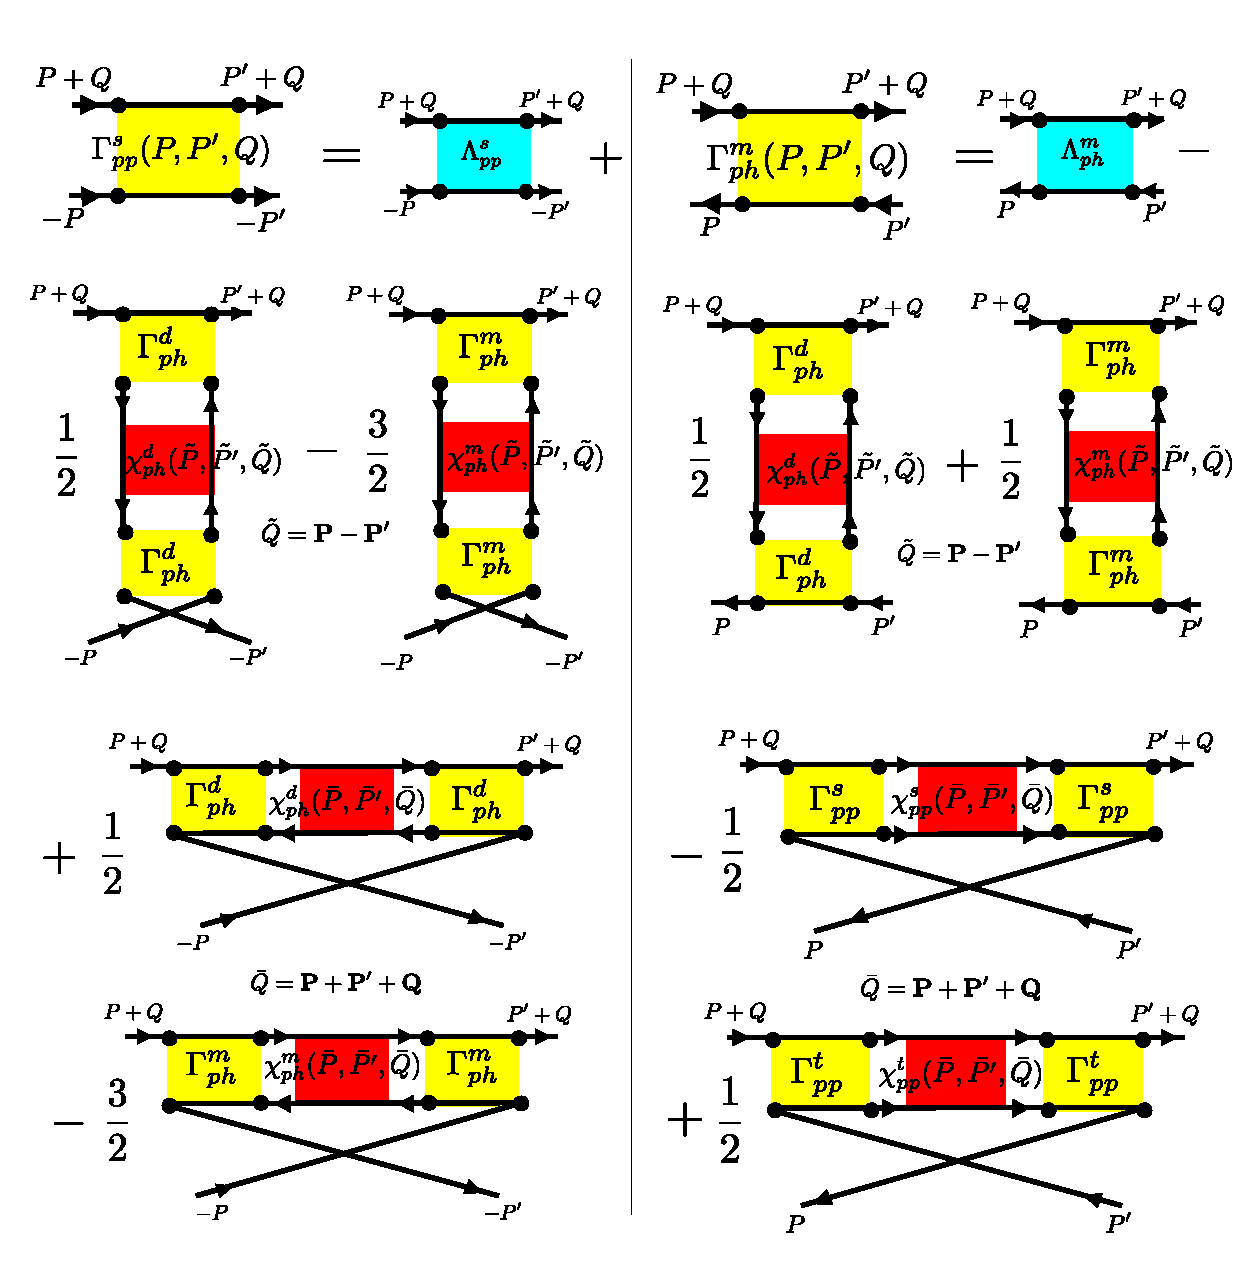
\includegraphics[width=\textwidth]{figure/parquet_pp_s_ph_m.pdf}
\caption{(Left panel) Parquet equation of the irreducible vertex function in the pp-s channel, $\Gamma^{s}_{pp}(P,P',Q)$. It is decomposed into a fully irreducible vertex function $\Lambda^{s}_{pp}$ and cross channel contributions from ph-d $\Phi^{d}_{ph}$, ph-m $\Phi^{m}_{ph}$ vertex ladders. The vertex ladders are products between irreducible vertex functions, $\Gamma$, and two-particle correlation functions, $\chi$, in the same channel, with the internal momentum-frequency indices being convoluted, but the momentum-frequency transfer determined by the indices of the irreducible vertex function in the LHS. (Right panel) Parquet equation for the irreducible vertex function in the ph-m channel, $\Gamma^{m}_{ph}(P,P',Q)$. Here the cross channel contributions also contain pp-s $\Phi^{s}_{pp}$ and pp-t $\Phi^{t}_{pp}$, vertex ladders.} \label{fig:parquet_pp_ph}
\end{figure}

CT-HYB/DMFT simulation is a powerful tool to obtain single-particle information. At the two-particle level, however, the correlation function $\chi(\omega,\omega',\nu)$ (which is the generalized susceptibility) and the irreducible vertex functions $\Gamma(\omega,\omega',\nu)$, can only be computed on the impurity site. Hence, the single-site CT-HYB/DMFT technique cannot capture non-local correlation effects of the underlying correlated lattice system. For example, the local particle-particle pairing susceptibilities can provide the information that the system has a superconducting instability in a certain parameter range, but one cannot access the pairing symmetry as the pairing susceptibilities do not have the necessary momentum information. This is an intrinsic limitation of the DMFT method~\cite{RevModPhys.68.13,RevModPhys.77.1027,RevModPhys.78.865}. 

To overcome this difficulty, we develop a new method to go beyond the local nature of DMFT, dubbed DMFT + Parquet formalism~\cite{Meng14a,Meng14b}. We take the local vertex and correlation functions computed in the CT-HYB/DMFT simulations, and bring in the momentum-dependence via two-particle level self-consistent diagrammatic relations -- the Parquet and Bethe-Salpeter equations. The obtained vertex and correlation functions are both momentum- and frequency-dependent. The Parquet equations relate the irreducible vertex function in one interaction channel to those in other channels~\cite{Dominicis64a,Dominicis64b}. Usually, we consider four interaction channels: the particle-hole density (ph-d), particle-hole magnetic (ph-m), particle-particle singlet (pp-s), and particle-particle triplet (pp-t) channels~\cite{PhysRevB.43.8044,PhysRevE.80.046706,PhysRevB.86.125114,PhysRevE.87.013311,PhysRevB.88.041103,PhysRevB.88.245110}. 

In the left (right) panel of Fig.~\ref{fig:parquet_pp_ph}, the Parquet equation in pp-s (ph-m) channels is shown. One sees that the irreducible vertex function in the pp-s (or ph-m) channel, $\Gamma^{s}_{pp}(P,P',Q)$ [or $\Gamma^{m}_{ph}(P,P',Q)$], can be decomposed into a fully irreducible vertex function, $\Lambda^{s}_{pp}(P,P',Q)$ [or $\Lambda^{m}_{ph}(P,P',Q)$], and vertex ladders in the ph-d channels [$\Phi^{d}_{ph}(-P',P+Q,P'-P)$ and $\Phi^{d}_{ph}(-P',-P,P+P'+Q)$] and ph-m channels [$\Phi^{m}_{ph}(-P',P+Q,P'-P)$ and $\Phi^{m}_{ph}(-P',-P,P+P'+Q)$]. Note that in the case of $\Gamma^{m}_{ph}(P,P',Q)$, the vertex ladders in the ph-d $\Phi^{d}_{ph}(P,P+Q,P'-P)$, ph-m $\Phi^{m}_{ph}(P,P+Q,P'-P)$, pp-s $\Psi^{s}_{pp}(-P-Q,-P,P+P'+Q)$ and pp-t $\Psi^{t}_{pp}(-P-Q,-P,P+P'+Q)$ channels need to be considered. Here $P\equiv(\mathbf{k},\omega)$, $P'\equiv(\mathbf{k'},\omega')$, and $Q\equiv(\mathbf{q},\nu)$, are all momentum-frequency 4-vectors. The rearrangement of the momentum-frequency indices of each vertex ladder is to respect the momentum and energy conservations for the scattering events.

From the lattice Green's function $G(P)$ and local irreducible vertex function $\Gamma(\omega,\omega',\nu)$ obtained in CT-HYB/DMFT, we construct the bubble term $\chi_0(P,Q)$ and then introduce the momentum transfer $\mathbf{q}$ to the two-particle correlation function, via the Bethe-Salpeter equation (BSE), 
\begin{equation}
\chi(\omega,\omega',Q)^{-1} = \left[\frac{1}{N\beta}\sum_{P}\chi_0(P,Q)\right]^{-1} - \Gamma(\omega,\omega',\nu).
\end{equation}
 We prepare such $\chi^{d/m}_{ph}(\omega,\omega',Q)$ and $\chi^{s/t}_{pp}(\omega,\omega',Q)$, along with the local irreducible vertex functions $\Gamma^{d/m}_{ph}(\omega, \omega',\nu)$ and $\Gamma^{s/t}_{pp}(\omega,\omega',\nu)$, insert them to the right-hand-side (RHS) of the Parquet equations in Fig.~\ref{fig:parquet_pp_ph}. Notice that we now have the information of $\tilde{Q}=P'-P$ and $\bar{Q}=P+P'+Q$ in the vertex ladders. Hence, for each fixed $Q$, we can construct the first order approximated irreducible vertex functions $\Gamma^{(1),d/m}_{ph}(P,P',Q)$ and $\Gamma^{(1),s/t}_{pp}(P,P',Q)$ in the left-hand-side (LHS) of the Parquet equations in Fig.~\ref{fig:parquet_pp_ph}.

The obtained irreducible vertex functions, $\Gamma^{(1),d/m}_{ph}(P,P',Q)$ and $\Gamma^{(1),s/t}_{pp}(P,P',Q)$, are the first order quantities in a two-particle self-consistent formulation. In the construction of the vertex ladders in Fig.~\ref{fig:parquet_pp_ph}, we approximate the momentum-frequency convolutions by frequency-only ones, as the input vertex functions are local. To complete the two-particle self-consistent calculation, we then iterate $\Gamma^{(1),d/m}_{ph}(P,P',Q)$ and $\Gamma^{(1),s/t}_{pp}(P,P',Q)$ back to Bethe-Salpeter and Parquet equations to generate the higher order two-particle irreducible vertex and correlation functions, in a successive manner. 

With the irreducible vertex functions at hand, we can study the various instabilities of the system generated by the electronic interactions, for example, the superconducting instabilities can be analyzed via the gap equation, 
\begin{equation}
\label{eq:gapeq}
\sum_{P'}\Gamma^{s/t}_{pp}(P,P',Q)\chi^{pp}_0(P',Q)\phi(P') = \lambda \phi(P),
\end{equation}
where the leading eigenvalue (LEV) $\lambda$ and the leading eigenvector $\phi(P)$ reveal the pairing information. Since $\Gamma^{s/t}_{pp}(P,P',Q)\chi^{pp}_{0}(P',Q)$ is the effective pairing interaction, as temperature approaches the transition temperature $T_{c}$, $\lambda \to 1$, and the leading eigenvector $\phi(P)$ reveals the momentum-dependence of the gap function~\cite{PhysRevB.88.041103,Meng14a,Meng14b}.

\section{Implementations and optimizations\label{sec:implement}}
\subsection{Development platform}
The main part of the $i$QIST software package was developed with the modern Fortran 90 language. We extensively used advanced language features in the Fortran 2003/2008 standard such as an object oriented programming style (polymorphic, inheritance, and module, etc.) to improve the readability and re-usability of the source codes. The compiler is fixed to the Intel Fortran compiler. We can not guarantee that the $i$QIST can be compiled successfully with other Fortran compilers. Some auxiliary scripts, pre- and post-processing tools are written using the Python language and Bash shell scripts. These scripts and tools act like a glue. They are very flexible and very easily extended or adapted to deal with various problems. In order to avoid incompatibilities, our Python codes only run on the Python 2.x runtime environment.

We use Git as the version control tool, and the source codes are hosted in a remote server. The developers pull the source codes from the server into their local machines, and then try to improve them. Once the development is done, the source codes can be pushed back to the server and merged with the master branch. Then the other developers can access them and use them immediately to start further developments. The members of our developer team can access the private code repository anywhere and anytime.  

\subsection{Orthogonal polynomial representation}
Boehnke \emph{et al.}~\cite{PhysRevB.84.075145} proposed that the Legendre polynomial can be used to improve the measurements of single-particle and two-particle Green's functions. Thanks to the Legendre polynomial representation, the numerical noise and memory space needed to store the Green's function are greatly reduced.

The imaginary time Green's function $G(\tau)$ is expressed using the Legendre polynomial $P_n(x)$ defined in [-1,1]:
\begin{equation}
\label{eq:gt_new}
G(\tau) = \frac{1}{\beta} \sum_{n \leq 0} \sqrt{2n + 1} P_{n}[x(\tau)] G_n,
\end{equation}
here $n$ is the order of Legendre polynomial, $G_{n}$ is the expansion coefficient, $x(\tau)$
maps $\tau \in [0,\beta]$ to $x \in [-1,1]$:
\begin{equation}
x(\tau) = \frac{2\tau}{\beta} - 1.
\end{equation}
Using the orthogonal relations of Legendre polynomials, we obtain 
\begin{equation}
\label{eq:gn_old}
G_n = \sqrt{2n + 1} \int^{\beta}_{0} d\tau P_{n}[x(\tau)] G(\tau).
\end{equation}
If we substitute Eq.~(\ref{eq:gt}) into Eq.~(\ref{eq:gn_old}), we get 
\begin{equation}
G_n = -\frac{\sqrt{2n + 1}}{\beta} \left\langle \sum^{k}_{i=1} \sum^{k}_{j=1}
\mathcal{M}_{ji} \tilde{P}_{n}(\tau^e_i - \tau^s_j) \right\rangle,
\end{equation}
where
\begin{equation}
\tilde{P}_n(\tau) = 
\begin{cases}
P_n [x(\tau)], & \tau > 0, \\
-P_n [x(\tau + \beta)], & \tau < 0, \\
\end{cases}
\end{equation}
and $\tau^{s}$ and $\tau^{e}$ denote the positions of creation and annihilation operators on the imaginary time axis, respectively. We can also express the Matsubara Green's function $G(i\omega_n)$ using Legendre polynomials:
\begin{equation}
\label{eq:gw_new}
G(i\omega_m) = \sum_{n \leq 0} T_{mn} G_n.
\end{equation}
The transformation matrix $T_{mn}$ is defined as
\begin{equation}
T_{mn} = (-1)^m i^{n+1} \sqrt{2n + 1} j_n \left[\frac{(2m + 1)\pi}{2}\right],
\end{equation}
where $j_n(z)$ is the spheric Bessel function. Actually, in the Monte Carlo simulation, only the expansion coefficients $G_n$ are measured. When the calculation is finished, the final Green's function can be evaluated using Eq.~(\ref{eq:gt_new}) and Eq.~(\ref{eq:gw_new}). It is worthwhile to note that the $T_{mn}$ do not depend on the inverse temperature $\beta$, so that we can calculate and store the matrix elements beforehand to save computer time.

It is easily to extend this formalism to other orthogonal polynomials. For example, in the $i$QIST software package, we not only implemented the Legendre polynomial representation, but also the Chebyshev polynomial representation. In the Chebyshev polynomial representation, the imaginary time Green's function $G(\tau)$ is expanded as follows:
\begin{equation}
G(\tau) = \frac{2}{\beta} \sum_{n \leq 0} U_n [x({\tau})]G_{n},
\end{equation}
here the $U_n(x)$ denote the second kind Chebyshev polynomials and $x \in [-1,1]$. The equation for the expansion coefficients $G_n$ is:
\begin{equation}
G_n = -\frac{2}{\pi\beta} \left\langle  \sum^{k}_{i=1} \sum^{k}_{j=1} 
\mathcal{M}_{ji} 
\tilde{U}_{n}(\tau^e_i - \tau^s_j)
\sqrt{1 - \tilde{x}(\tau^e_i - \tau^s_j)^2}
\right\rangle,
\end{equation}
where
\begin{equation}
\tilde{U}_n (x) = 
\begin{cases}
U_n[x(\tau)], & \tau > 0, \\
-U_n[x(\tau+\beta)], & \tau < 0, \\
\end{cases}
\end{equation}
and
\begin{equation}
\tilde{x}(\tau) = 
\begin{cases}
x(\tau), & \tau > 0, \\
x(\tau + \beta), & \tau < 0. \\
\end{cases}
\end{equation}
Unfortunately, there is no explicit expression for $G(i\omega_n)$ [like Eq.~(\ref{eq:gw_new})] in the Chebyshev polynomial representation.

\subsection{Improved estimator for the self-energy function\label{subsec:self}}
Recently, Hafermann \emph{et al.} proposed efficient measurement procedures for the self-energy and vertex functions within the CT-HYB algorithm~\cite{PhysRevB.85.205106,PhysRevB.89.235128}. In their method, some higher-order correlation functions (related to the quantities being sought through the equation of motion) are measured. For the case of interactions of density-density type, the segment algorithm is available~\cite{PhysRevLett.97.076405}. Thus, the additional correlators can be obtained essentially at no additional computational cost. When the calculations are completed, the required self-energy function and vertex function can be evaluated analytically.

The improved estimator for the self-energy function can be expressed in the following form:
\begin{equation}
\label{eq:self-energy}
\Sigma_{ab}(i\omega_n) = \frac{1}{2} 
\sum_{ij} G^{-1}_{ai}(i\omega_n) (U_{jb} + U_{bj}) F^{j}_{ib}(i\omega_n),
\end{equation}
where $U_{ab}$ is the Coulomb interaction matrix element. The expression for the new two-particle correlator $F^{j}_{ab}(\tau - \tau')$ reads
\begin{equation}
F^{j}_{ab}(\tau-\tau') 
= -\langle \mathcal{T} d_{a}(\tau) d^{\dagger}_{b}(\tau') n_{j}(\tau') \rangle,
\end{equation}
and $F^{j}_{ab}(i\omega_n)$ is its Fourier transform. The actual measurement formula is
\begin{equation}
F^{j}_{ab}(\tau - \tau') = 
-\frac{1}{\beta}
\left\langle
\sum_{\alpha\beta = 1}^{k} 
\mathcal{M}_{\beta\alpha}\delta^{-}(\tau-\tau', \tau^{e}_{\alpha} - \tau^{s}_{\beta})
n_{j}(\tau^s_\beta)\delta_{a,\alpha}\delta_{b,\beta}
\right\rangle.
\end{equation}
As one can see, this equation looks quite similar to Eq.~(\ref{eq:gt}). Thus we use the same method to measure $F^{j}_{ab}(\tau - \tau')$ and finally get the self-energy function via Eq.~(\ref{eq:self-energy}). Here, the matrix element $n_{j}(\tau^s_\beta)$ (one or zero) denotes whether or not flavor $j$ is occupied (whether or not a segment is present) at time $\tau^s_\beta$.

This method can be combined with the orthogonal polynomial representation~\cite{PhysRevB.84.075145} as introduced in the previous subsection to suppress fluctuations and filter out the Monte Carlo noise. Using this technique, we can obtain the self-energy and vertex functions with unprecedented accuracy, which leads to an enhanced stability in the analytical continuations of those quantities~\cite{PhysRevB.85.205106}. In the $i$QIST software package, we only implemented the improved estimator for the self-energy function. Note that when the interaction matrix is frequency-dependent, Eq.~(\ref{eq:self-energy}) should be modified slightly~\cite{PhysRevB.89.235128}.

\subsection{Random number generators}
Fast, reliable, and long period pseudo-random number generators are a key factor for any Monte Carlo simulations. Currently, the most popular random number generator is the Mersenne Twister which was developed in 1998 by Matsumoto and Nishimura~\cite{Matsumoto:1998}. Its name derives from the fact that its period length is chosen to be a Mersenne prime. In the $i$QIST software package, we implemented the commonly used version of Mersenne Twister, MT19937. It has a very long period of $2^{19937}-1$. Of course, if we choose different parameter sets, its period can be shorter or longer.

The Mersenne Twister is a bit slow by today's standards. So in 2006, a variant of Mersenne Twister, the SIMD-oriented Fast Mersenne Twister (SFMT) was introduced~\cite{sfmt:2008}. It was designed to be fast when it runs on 128-bit SIMD. It is almost twice as fast as the original Mersenne Twister and has better statistics properties. We also implemented it in the $i$QIST software package, and use it as the default random number generator.

The $i$QIST software package offers other excellent generators as well, such as WELL (Well Equidistributed Long-period Linear)~\cite{Panneton:2006} and Marsaglia's XORSHIFT generators~\cite{Marsaglia:2003}, etc. The XORSHIFT generator is the fastest.

\subsection{Subspaces and symmetry\label{subsec:subspace}}
For a local Hamiltonian $H_{\text{loc}}$ with general interactions, the evaluation of local trace is heavily time-consuming,
\begin{equation}
\label{equ:tr1}
\omega_{d}(\mathcal{C}) = 
\text{Tr}_{\text{loc}} (T_{2k+1}F_{2k}T_{2k} \cdots F_{2}T_{2}F_{1}T_{1}),
\end{equation}  
where $T=e^{-\tau H_{\text{loc}}}$ is time evolution operator, $F$ is a fermion creation or annihilation operator, and $k$ is the expansion order for the current diagrammatic configuration $\mathcal{C}$. The straightforward method to evaluate this trace is to insert the complete eigenstates $\{ \Gamma \}$ of $H_{\text{loc}}$ into the RHS of Eq.~(\ref{equ:tr1}), then 
\begin{eqnarray}\label{equ:tr2}
\text{Tr}_{\text{loc}} &= &\sum_{\{\Gamma_{1}\Gamma_{2} \cdots \Gamma_{2k}\}} 
            \langle\Gamma_{1}|T_{2k+1}|\Gamma_{1}\rangle
            \langle\Gamma_{1}|F_{2k}|\Gamma_{2k}\rangle
            \langle\Gamma_{2k}|T_{2k}|\Gamma_{2k}\rangle \cdots \nonumber \\  
          & &\times \langle\Gamma_{3}|F_{2}|\Gamma_{2}\rangle
            \langle\Gamma_{2}|T_{2}|\Gamma_{2}\rangle
            \langle\Gamma_{2}|F_{1}|\Gamma_{1}\rangle
            \langle\Gamma_{1}|T_{1}|\Gamma_{1}\rangle.
\end{eqnarray}
Thus, we must do $4k+1$ matrix-matrix multiplications with the dimension of the Hilbert space of $H_{\text{loc}}$. This method is robust but very slow for large multi-orbital impurity model as the dimension of the matrix is impractically large for 5- and 7-band systems, and the expansion order $k$ is large as well.

Actually, the matrices of the fermion operators ($F$-matrix) are very sparse due to the symmetry of $H_{\text{loc}}$. We can take advantage of this to speed up the matrix-matrix multiplications. We consider the symmetry of $H_{\text{loc}}$ to find some good quantum numbers (GQNs) and divide the full Hilbert space of $H_{\text{loc}}$ with very large dimension into much smaller subspaces labeled by these GQNs~\cite{RevModPhys.83.349}. We call a subspace $|\alpha\rangle$ as a superstate~\cite{PhysRevB.75.155113} which consists of all the $n_{\alpha}$ eigenstates of this subspace, $|\alpha\rangle=\{ \Gamma_{1}, \Gamma_{2}, \cdots, \Gamma_{n_{\alpha}}\}$. The $F$-matrix element can only be nonzero between pairs of superstates with different values of GQNs. One fermion operator may bring one initial superstate $|\alpha\rangle$ to some other final superstates $|\beta\rangle$,
\begin{equation}\label{equ:next_sect}
F|\alpha\rangle= |\beta\rangle,
\end{equation}
or outside of the full Hilbert space. We have to carefully choose some GQNs to make sure that for a fixed initial superstate $|\alpha\rangle$ and a fixed fermion operator, there is one and only one final superstate $|\beta\rangle$ if it doesn't go outside of the full Hilbert space. Given an arbitrary diagrammatic configuration, starting with a superstate $|\alpha_{1}\rangle$, there will be only one possible evolution path. That is,
\begin{equation}
|\alpha_{1}\rangle \xrightarrow{F_{1}} 
|\alpha_{2}\rangle \xrightarrow{F_{2}} 
|\alpha_{3}\rangle \xrightarrow{F_{3}} 
|\alpha_{4}\rangle \cdots 
|\alpha_{2k-1}\rangle \xrightarrow{F_{2k-1}} 
|\alpha_{2k}\rangle   \xrightarrow{F_{2k}} 
|\alpha_{1}\rangle.
\end{equation}
The path may break at some point because it goes outside of the full Hilbert space or violates the Pauli principle. For a successful path starting with $|\alpha_{1}\rangle$, its contribution to the local trace is
\begin{eqnarray}
\text{Tr}_{\alpha_{1}} &=& 
\sum_{\{ \Gamma_{\alpha_{1}}, \Gamma_{\alpha_{2}}, \cdots, \Gamma_{\alpha_{2k}}\}}
\langle\Gamma_{\alpha_{1}}|T_{2k+1}|\Gamma_{\alpha_{1}}\rangle
\langle\Gamma_{\alpha_{1}}|F_{2k}|\Gamma_{\alpha_{2k}}\rangle
\langle\Gamma_{\alpha_{2k}}|T_{2k}|\Gamma_{\alpha_{2k}}\rangle \cdots \nonumber \\ 
& & \times 
\langle\Gamma_{\alpha_{3}}|F_{2}|\Gamma_{\alpha_{2}}\rangle
\langle\Gamma_{\alpha_{2}}|T_{2}|\Gamma_{\alpha_{2}}\rangle
\langle\Gamma_{\alpha_{2}}|F_{1}|\Gamma_{\alpha_{1}}\rangle
\langle\Gamma_{\alpha_{1}}|T_{1}|\Gamma_{\alpha_{1}}\rangle,
\end{eqnarray}
where $\{ \Gamma_{\alpha_{i}} \}$ are the eigenstates of subspace $\alpha_{i}$. Thus, the final local trace should be
\begin{equation}
\text{Tr}_{\text{loc}} = \sum_{i} \text{Tr}_{\alpha_{i}}.
\end{equation} 
As a result, the original $4k+1$ matrix-matrix multiplications with large dimension reduces to several $4k+1$ matrix-matrix multiplications with much smaller dimensions, resulting in a huge speedup.

\begin{table}[t]
\caption{The GQNs supports for various types of local Hamiltonians $H_{\text{loc}}$. \label{table:good}}
\centering
\begin{tabular}{cccc}
\hline
\hline
 GQNs                   & Kanamori-$U$ & Slater-$U$ &  SOC \\
\hline
$N, S_{z}$              & Yes          & Yes        & No   \\ 
$N, S_{z}$, PS          & Yes          & No         & No   \\ 
$N, J_{z}$              & Yes          & Yes        & Yes  \\
$N$                     & Yes          & Yes        & Yes  \\ 
\hline
\hline
\end{tabular}
\end{table}

In our codes, we implemented several GQNs schemes for different types of local Hamiltonians $H_{\text{loc}}$, which is summarized in Table~\ref{table:good}. For $H_{\text{loc}}$ without spin-orbit coupling (SOC), we have two choices: (1) with Slater parameterized Coulomb interaction matrix, we use the total occupation number $N$, the $z$ component of total spin $S_{z}$ as GQNs; (2) with Kanamori parameterized Coulomb interaction matrix, besides $N$ and $S_{z}$, we can use another powerful GQN, the so-called PS number~\cite{PhysRevB.86.155158}. It is defined as,
\begin{equation}
\text{PS} = \sum_{\alpha=1}^{N_{\text{orb}}} \\
             (n_{\alpha\uparrow}-n_{\alpha\downarrow})^2 \times 2^{\alpha},
\end{equation}
where $\alpha$ is the orbital index, $\{\uparrow, \downarrow\}$ is spin index, $n_{\alpha\uparrow}$ and $n_{\alpha\downarrow}$ are the orbital occupancy numbers. The PS number labels the occupation number basis with the same singly occupied orbitals. With its help, the dimensions of the subspaces become very small, such that we can treat 5-band Kanamori systems efficiently without any approximations. For $H_{\text{loc}}$ with SOC, we can use the total occupancy number $N$ and the $z$ component of total angular momentum $J_{z}$ as GQNs. We summarize the total number of subspaces, maximum and mean dimension of subspaces for different GQNs schemes and multi-orbital impurity models in Table.~\ref{table:dim}. Obviously, using these GQNs can largely reduce the dimension of the $F$-matrix, and make accurate DMFT calculations for complex electronic systems (such as $d$- and $f$-electron materials) possible. 

\begin{table}[t]
\caption{The total number of subspaces $N$, maximum and mean dimension of subspaces for different GQNs schemes and multi-orbital models. \label{table:dim}} 
\centering
\begin{tabular}{ccccc}
\hline
\hline
                & 2-band       & 3-band       & 5-band       & 7-band          \\
\hline
GQNs            & $N$/max/mean & $N$/max/mean & $N$/max/mean & $N$/max/mean    \\ 
\hline
$N, S_{z}$      &  9/4/1.78    & 16/9/4.00    & 36/100/28.44 & 64/1225/256.00  \\
$N, S_{z}$, PS  &  14/2/1.14   & 44/3/1.45    & 352/10/2.91  & 2368/35/6.92    \\
$N, J_{z}$      &  -           & 26/5/2.46    & 96/37/10.67  & 246/327/66.60   \\
$N$             &  5/6/3.20    & 7/20/9.14    & 11/252/93.09 & 15/3432/1092.27 \\ 
\hline
\hline
\end{tabular}
\end{table}

\subsection{Truncation approximation}
As discussed in Sec.~\ref{subsec:subspace}, although we have used GQNs to split the full Hilbert space with very large dimension into blocks with smaller dimensions [for cases such as 7-band systems with GQNs ($N$, $J_{z}$) and 5-band systems with GQN ($N$)], the dimensions of some blocks are still too large and the numbers of blocks are too much so that it is still very expensive to evaluate the local trace. Haule proposed in Ref.~\cite{PhysRevB.75.155113} to discard some high-energy states because they are rarely visited. For example, for 7-band system with only 1 electron (like Ce metal), only states with occupancy $N=0$, 1, 2 will be frequently visited, and states with occupancy $N>2$ can be truncated completely to reduce the large Hilbert space to a very small one. Of course, this truncation approximation may cause some bias because a frequently visited state may be accessed via an infrequently visited state. Therefore, one should be cautious when adopting the truncation approximation, and for example run some convergence tests. 

Currently, we adopted two truncation schemes in our codes. The first scheme relies on the occupation number. We just keep those states whose occupation numbers are close to the nominal valence and skip the other states, as shown in the above example. This scheme is quite robust if the charge fluctuations are small enough, such as in the case of a Mott insulating phase. Another scheme is to dynamically truncate the states with very low probability based on statistics which is recorded during the Monte Carlo sampling. This scheme is not very stable, so one needs to use it with caution.

\subsection{Lazy trace evaluation}
The diagrammatic Monte Carlo sampling algorithm consists of the following steps: (1) Propose an update for the current diagrammatic configuration. (2) Calculate the acceptance probability $p$ according to the Metropolis-Hasting algorithm,
\begin{equation}
p = \text{min} (1, \frac{A^\prime}{A} \left| \frac{\omega_{c}}{\omega_{c}^{\prime}}\right| 
     \left|\frac{\omega_{d}}{\omega_{d}^{\prime}} \right|),
\end{equation}
where, $A$ is the proposal probability for the current update and $A^\prime$ for the inverse update, $\omega_{c}$ and $\omega_{c}^{\prime}$ are the determinants for the new and old configurations, respectively, and $\omega_{d}$ and $\omega_{d}^{\prime}$ are the local traces for the new and old configurations, respectively. (3) Generate a random number $r$. If $p>r$, the proposed update is accepted, otherwise it is rejected. (4) Update the current diagrammatic configuration if the proposed update is accepted. It turns out that for CT-HYB, $p$ is usually low ($1\% \sim 20\%$), especially in the low temperature region. On the other hand, the calculation of $p$ involves a costly local trace evaluation. To avoid wasting computation time when the acceptance probability is very low, in the subspace algorithm, we implemented the so-called lazy trace evaluation proposed in Ref.~\cite{arXiv:1403.7214}.

 The basic idea of the lazy trace evaluation is simple. For the proposed Monte Carlo move, we first generate a random number $r$. Then, instead of calculating the local trace from scratch to determine $p$, we calculate bounds for $\left|\text{Tr}_{\text{loc}}\right|$,
\begin{equation}
\left|\omega_{d}\right| = \left|\text{Tr}_{\text{loc}}\right| \leq \sum_{i} \left|\text{Tr}_{i}\right| \leq \sum_{i} B_{i},
\end{equation}
where $B_i \geq \left|\text{Tr}_{i}\right|$. $B_{i}$ is a product of some chosen matrix norms of $T$ and $F$ matrices: 
\begin{equation}
B_i = C  \left\| T_{2k+1} 
\right\| \left\| F_{2k} \right\| \cdots \left\| F_{2} \right\| \left\| T_{2} \right\| 
\left\| F_{1} \right\| \left\| T_{1} \right\| \geq
\left|\text{Tr}(T_{2k+1}F_{2k} \cdots F_{2}T_{2}F_{1}T_{1})\right|,
\end{equation}
where $C$ is a parameter depending on the specific type of matrix norm, and $\left\| \cdot \right\|$ denotes a matrix norm.
If $\text{Tr}_{i^\prime}$ denotes the exact trace of some subspaces, then we have 
\begin{equation}
\left| \left|\text{Tr}_{\text{loc}}\right| - \sum_{i^\prime}\left|\text{Tr}_{i^\prime}\right| \right| 
\leq \sum_{i \neq i^\prime} B_{i}.
\end{equation}
Thus, we can determine the upper $p_{\text{max}}$ and lower $p_{\text{min}}$ bounds of $p$ as
\begin{equation}
\begin{aligned}
p_{\text{max}}=R \left(\sum_{i^\prime}\left|\text{Tr}_{i^\prime}\right| + \sum_{i \neq i^\prime} B_{i}\right),\\
p_{\text{min}}=R \left(\sum_{i^\prime}\left|\text{Tr}_{i^\prime}\right| - \sum_{i \neq i^\prime} B_{i}\right),
\end{aligned}
\end{equation} 
where $R=\frac{A^\prime}{A} \left| \frac{\omega_{c}}{\omega_{c}^{\prime}}\right| \left|\frac{1}{\omega_{d}^{\prime}} \right|$.
If $r>p_{\text{max}}$, we reject this move immediately. If $r<p_{\text{min}}$, we accept the move and calculate the determinant and local trace from scratch. If $ p_{\text{min}} < r < p_{\text{max}} $, we refine the bounds by calculating the local trace of one more subspace $\text{Tr}_{i}$ until we can reject or accept the move. The calculation of these bounds involves only simple linear algebra calculations of matrix norms which cost little computation time, and one refining operation involves only one subspace trace evaluation. On average, it saves a lot of computation time, as confirmed by our benchmarks.

\subsection{Divide-and-conquer and sparse matrix tricks}
\begin{figure}[tp]
\centering
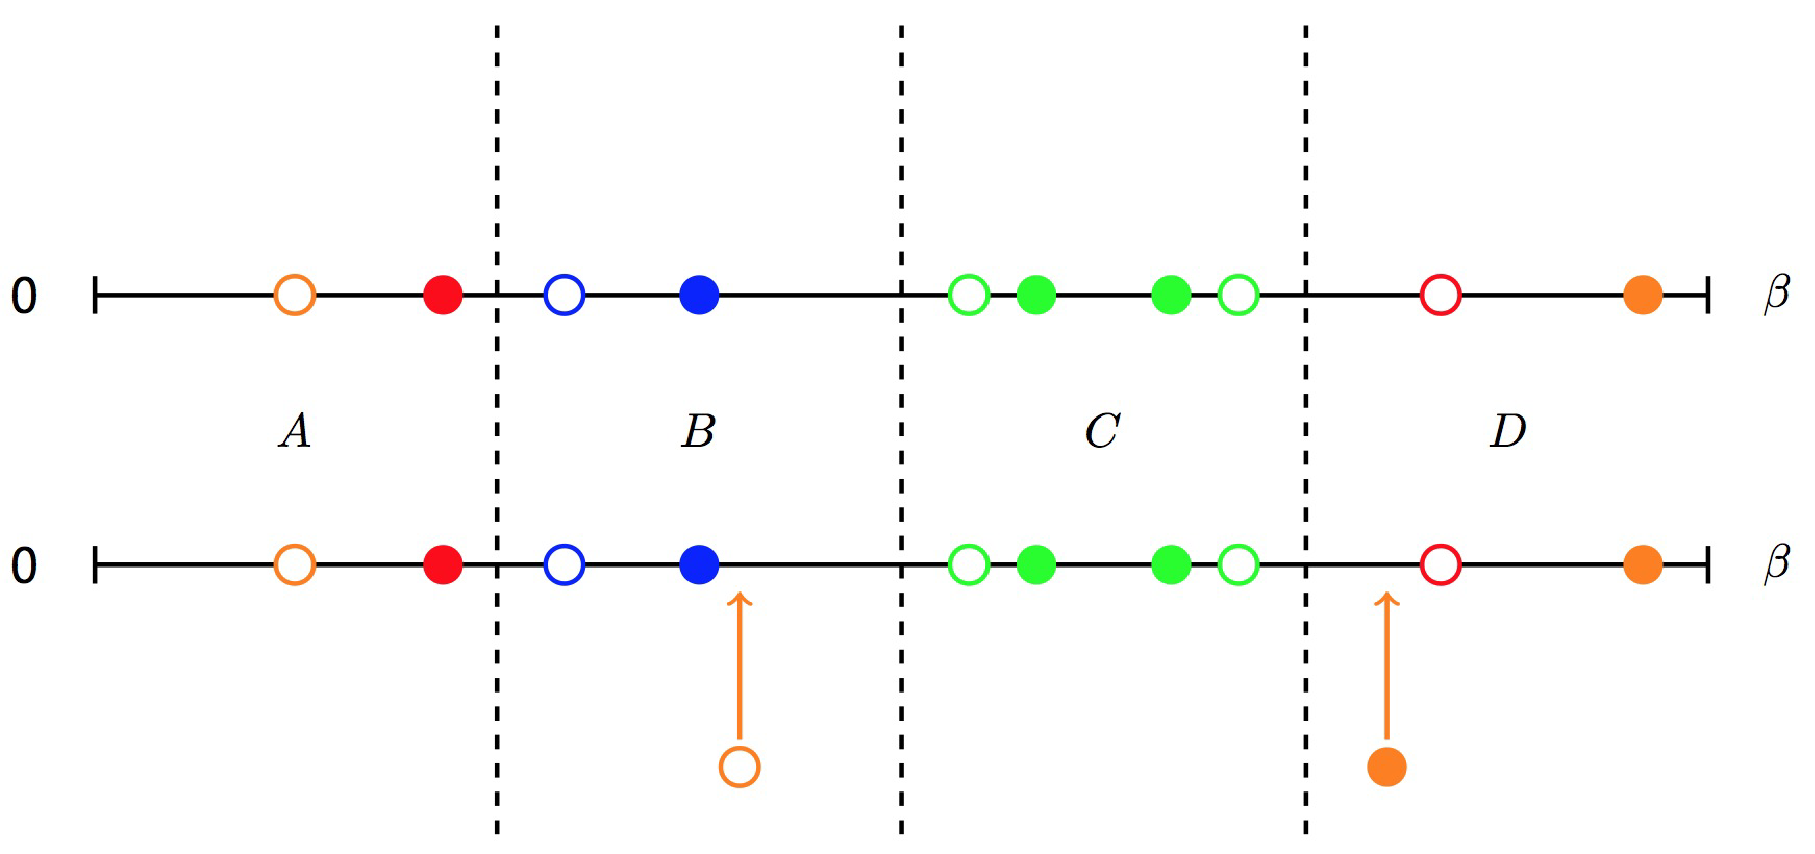
\includegraphics[width=1.0\textwidth]{figure/divide.pdf}
\caption{Illustration of the divide-and-conquer algorithm. The imaginary time axis is split into four parts with equal length by vertical dashed lines. The open (filled) circles mean creation (annihilation) operators. The color is used to distinguish different flavors. It shows that a creation operator is inserted into the $B$ part, while a annihilation operator is inserted into the $D$ part. \label{fig:div}}
\end{figure}

The Monte Carlo updates, such as inserting (removing) a pair of creation and annihilation operators, usually modify the diagrammatic configuration locally. Based on this fact, we implemented a divide-and-conquer algorithm to speed up the trace evaluation. As illustrated in Fig.~\ref{fig:div}, we divide the imaginary time axis into a few parts with equal length. For each part, there will be zero or nonzero fermion operators, and we save their matrix products when evaluating the local trace in the beginning. In the next Monte Carlo sampling, we first determine which parts may be modified or influenced, and then for these parts we recalculate the matrix products from scratch and save them again. For the unchanged parts, we will leave them unchanged. Finally, we will multiply the contributions of all parts to obtain the final local trace. By using this divide-and-conquer trick, we can avoid redundant computations and speed up the calculation of the acceptance probability $p$. This trick can be combined with the GQNs algorithm to achieve a further speedup. 

If direct matrix-matrix multiplications are used when evaluating the local trace, the $F$-matrix must be very sparse. Thus, we can convert them into sparse matrices in compressed sparse row (CSR) format, and then the sparse matrix multiplication can be applied to obtain a significant speedup.

\subsection{Parallelization}
All of the CT-HYB impurity solvers in the $i$QIST software package are parallelized by MPI. The strategy is very simple. In the beginning, we launch $n$ processes simultaneously. The master process is responsible for reading input data and configuration parameters, and broadcasts them among the children processes, and then each process will perform Monte Carlo samplings and measure physical observables independently. After all the processes finish their jobs, the master process will collect the measured quantities from all the processes and average them to obtain the final results. Apart from that, no additional inter-process communication is needed. Thus, we can anticipate that the parallel efficiency will be very good, and near linear speedups are possible, as long as the number of thermalization steps is small compared to the total number of Monte Carlo steps. 

In practical calculations, we always fix the number of Monte Carlo steps $N_{\text{sweep}}$ done by each process, and launch as many processes as possible. Suppose that the number of processes is $N_{\text{proc}}$, then the total number of Monte Carlo samplings should be $N_{\text{proc}}N_{\text{sweep}}$. Naturally, the more processes we use, the more accurate data we can obtain.

\section{Atomic Solver}
The $\mathcal{J}asmine$ component of $i$QIST is used to solve a local atomic Hamiltonian defined as,

\begin{equation}
\hat{H}_{\text{atom}}=\hat{H}_{0}+\hat{H}_{U},
\end{equation}
where, $\text{\ensuremath{\hat{H}}}_{0}$ is the on-site term, including
crystal field (CF) splitting term $\hat{H}_{\text{CF}}$, spin-orbit
coupling (SOC) term $\hat{H}_{\text{SOC}}$, and other terms such
as a Zeeman term in case of the presence of external magnetic field,

\begin{equation}
\hat{H}_{0}=\hat{H}_{\text{CF}}+\hat{H}_{\text{SOC}}+\text{other on-site terms},
\end{equation}
and $\hat{H}_{U}$ is the Coulomb interaction term.

We write these terms in second quantization form, 

\begin{equation}
\hat{H}_{\text{atom}}=\sum_{\alpha,\beta}E_{\alpha,\beta}\hat{f}_{\alpha}^{\dagger}\hat{f}_{\beta}+\sum_{\alpha,\beta,\gamma,\delta}U_{\alpha,\beta,\gamma,\delta}\hat{f}_{\alpha}^{\dagger}\hat{f}_{\beta}^{\dagger}\hat{f}_{\delta}\hat{f}_{\gamma},
\end{equation}
where, $\alpha,\beta,\gamma,\delta$ is the single particle orbital-spin
index, the first term is the on-site term, the second one is the Coulomb
interaction term.


\subsection{Definition of single particle basis}

In this section, we define some single particle basis we used in $\mathcal{J}asmine$
to write down the atomic Hamiltonian $\hat{H}_{\text{atom}}$. We
set $\hbar=1$ in this note.


\subsubsection{complex spherical harmonics basis}

The complex shperical harmonics $Y_{l}^{m}(\theta,\phi)$ is the eigenstate
of $l^{2},l_{z}$,

\begin{equation}
l^{2}Y_{l}^{m}=l(l+1)Y_{l}^{m},
\end{equation}


\begin{equation}
l_{z}Y_{l}^{m}=mY_{l}^{m},\ m=-l,-l+1,\cdots,l.
\end{equation}



\subsubsection{real spherical harmonics basis}

The real spherical harmonics $Y_{lm}$ is defined as

\begin{gather}
Y_{lm}=\begin{cases}
\frac{i}{\sqrt{2}}\left(Y_{l}^{-|m|}-(-1)^{m}Y_{l}^{|m|}\right) & if\ m<0,\\
Y_{l}^{0} & if\ m=0,\\
\frac{1}{\sqrt{2}}\left(Y_{l}^{-|m|}+(-1)^{m}Y_{l}^{|m|}\right) & if\ m>0.
\end{cases}
\end{gather}
For $p$ system,

\begin{eqnarray}
p_{x} & = & Y_{11}=\frac{1}{\sqrt{2}}\left(Y_{1}^{-1}-Y_{1}^{1}\right),\nonumber \\
p_{y} & = & Y_{1,-1}=\frac{i}{\sqrt{2}}\left(Y_{1}^{-1}+Y_{1}^{1}\right),\\
p_{z} & = & Y_{10}=Y_{1}^{0}.\nonumber 
\end{eqnarray}
For $d$ system,

\begin{eqnarray}
d_{z^{2}} & = & Y_{20}=Y_{2}^{0},\nonumber \\
d_{zx} & = & Y_{21}=\frac{1}{\sqrt{2}}\left(Y_{2}^{-1}-Y_{2}^{1}\right),\nonumber \\
d_{zy} & = & Y_{2,-1}=\frac{i}{\sqrt{2}}\left(Y_{2}^{-1}+Y_{2}^{1}\right),\\
d_{x^{2}-y^{2}} & = & Y_{22}=\frac{1}{\sqrt{2}}\left(Y_{2}^{-2}+Y_{2}^{2}\right),\nonumber \\
d_{xy} & = & Y_{2,-2}=\frac{i}{\sqrt{2}}\left(Y_{2}^{-2}-Y_{2}^{2}\right).\nonumber 
\end{eqnarray}
For $t_{2g}$ system $(l\approx-1)$, we have a $T-P$ equivalence, 

\begin{eqnarray}
d_{zx} & \rightarrow & p_{y}=\frac{i}{\sqrt{2}}\left(Y_{1}^{-1}+Y_{1}^{1}\right),\nonumber \\
d_{zy} & \rightarrow & p_{x}=\frac{1}{\sqrt{2}}\left(Y_{1}^{-1}-Y_{1}^{1}\right),\\
d_{xy} & \rightarrow & p_{z}=Y_{1}^{0}.\nonumber 
\end{eqnarray}
For $f$ system, 

\begin{eqnarray}
f_{z^{3}} & = & Y_{30}=Y_{3}^{0},\nonumber \\
f_{xz^{2}} & = & Y_{31}=\frac{1}{\sqrt{2}}\left(Y_{3}^{-1}-Y_{3}^{1}\right),\nonumber \\
f_{yz^{2}} & = & Y_{3,-1}=\frac{i}{\sqrt{2}}\left(Y_{3}^{-1}+Y_{3}^{1}\right),\nonumber \\
f_{z(x^{2}-y^{2})} & = & Y_{32}=\frac{1}{\sqrt{2}}\left(Y_{3}^{-2}+Y_{3}^{2}\right),\\
f_{xyz} & = & Y_{3,-2}=\frac{i}{\sqrt{2}}\left(Y_{3}^{-2}-Y_{3}^{2}\right),\nonumber \\
f_{x(x^{2}-3y^{2})} & = & Y_{33}=\frac{1}{\sqrt{2}}\left(Y_{3}^{-3}-Y_{3}^{3}\right),\nonumber \\
f_{y(3x^{2}-y^{2})} & = & Y_{3,-3}=\frac{i}{\sqrt{2}}\left(Y_{3}^{-3}+Y_{3}^{3}\right).\nonumber 
\end{eqnarray}



\subsubsection{cubic spherical harmonics basis}

The cubic shperical harmonics is defined as the basis of the irreducible
representation of cubic point group $O_{h}$.

$p$ orbitals:

\begin{equation}
T_{1u}:p_{x},p_{y},p_{z}
\end{equation}


$d$ orbitals:

\begin{gather}
\begin{cases}
E_{g}: & d_{z^{2}},d_{x^{2}-y^{2}}\\
T_{2g}: & d_{zx},d_{zy},d_{xy}
\end{cases}
\end{gather}


$f$ orbitals:

\begin{eqnarray}
f_{x^{3}} & = & -\frac{\sqrt{6}}{4}f_{xz^{2}}+\frac{\sqrt{10}}{4}f_{x(x^{2}-3y^{2})}\nonumber \\
f_{y^{3}} & = & -\frac{\sqrt{6}}{4}f_{yz^{2}}-\frac{\sqrt{10}}{4}f_{y(3x^{2}-y^{2})}\nonumber \\
f_{z^{3}} & = & f_{z^{3}}\nonumber \\
f_{x(y^{2}-z^{2})} & = & -\frac{\sqrt{10}}{4}f_{xz^{2}}-\frac{\sqrt{6}}{4}f_{x(x^{2}-3y^{2})}\\
f_{y(z^{2}-x^{2})} & = & \frac{\sqrt{10}}{4}f_{yz^{2}}-\frac{\sqrt{6}}{4}f_{y(3x^{2}-y^{2})}\nonumber \\
f_{z(x^{2}-y^{2})} & = & f_{z(x^{2}-y^{2})}\nonumber \\
f_{xyz} & = & f_{xyz}\nonumber 
\end{eqnarray}


\begin{gather}
\begin{cases}
T_{1u}: & f_{x^{3}},f_{y^{3}},f_{z^{3}}\\
T_{2u}: & f_{x(y^{2}-z^{2})},f_{y(z^{2}-x^{2})},f_{z(x^{2}-y^{2})}\\
A_{2u}: & f_{xyz}
\end{cases}
\end{gather}



\subsubsection{$j^{2},j_{z}$ diagonal basis}

Define $\phi_{ljm_{j}}$ as the eigenstate of $j^{2},j_{z}$,

\begin{equation}
j^{2}\phi_{ljm_{j}}=j(j+1)\phi_{ljm_{j}},
\end{equation}


\begin{equation}
j_{z}\phi_{ljm_{j}}=m_{j}\phi_{ljm_{j}}.
\end{equation}


For $j=l+\frac{1}{2},m_{j}=m+\frac{1}{2}$,

\begin{equation}
\phi_{ljm_{j}}=\sqrt{\frac{l+m+1}{2l+1}}Y_{l}^{m}\uparrow+\sqrt{\frac{l-m}{2l+1}}Y_{l}^{m+1}\downarrow.
\end{equation}


For $j=l-\frac{1}{2},m_{j}=m+\frac{1}{2}$,

\begin{equation}
\phi_{ljm_{j}}=-\sqrt{\frac{l-m}{2l+1}}Y_{l}^{m}\uparrow+\sqrt{\frac{l+m+1}{2l+1}}Y_{l}^{m+1}\downarrow.
\end{equation}



\subsubsection{Natural basis}

The natural basis is defined as the diagonal basis of on-site term
$E_{\alpha\beta}$.


\subsection{Spin-orbit coupling}

The spin-orbit coupling (SOC) is implemented at atomic level, 

\begin{equation}
\hat{H}_{\text{SOC}}=\lambda\sum_{i}\vec{\mathbf{l}}_{i}\cdot\vec{\mathbf{s}}_{i},
\end{equation}


where, $\vec{\mathbf{l}}$ is orbital angular momentum, and $\vec{\mathbf{s}}$
is spin angular momentum. 

In second quantization form,

\begin{equation}
\hat{H}_{\text{SOC}}=\lambda\sum_{\alpha\sigma,\beta\sigma^{\prime}}\Braket{\alpha\sigma|\vec{\mathbf{l}}\cdot\vec{\mathbf{s}}|\beta\sigma^{\prime}}\hat{f}_{\alpha\sigma}^{\dagger}\hat{f}_{\beta\sigma^{\prime}},
\end{equation}


where, $\alpha$ is orbital index and $\sigma$ is spin index, and 

\begin{eqnarray}
\vec{\mathbf{l}}\cdot\vec{\mathbf{s}} & = & \frac{1}{2}\vec{\mathbf{l}}\cdot\vec{\mathbf{\mathbf{\sigma},}}
\end{eqnarray}


where, $\vec{\mathbf{\sigma}}$ is Pauli operator.

\begin{eqnarray*}
\end{eqnarray*}
\begin{eqnarray*}
\vec{\mathbf{l}}\cdot\vec{\mathbf{\sigma}} & = & \hat{l}_{x}\hat{\sigma}_{x}+\hat{l}_{y}\hat{\sigma}_{y}+\hat{l}_{z}\hat{\sigma}_{z}\\
 & = & \left[\begin{array}{cc}
0 & \hat{l}_{x}\\
\hat{l}_{x} & 0
\end{array}\right]+\left[\begin{array}{cc}
0 & -i\hat{l}_{y}\\
i\hat{l}_{y} & 0
\end{array}\right]+\left[\begin{array}{cc}
\hat{l}_{z} & 0\\
0 & -\hat{l}_{z}
\end{array}\right]\\
 & = & \left[\begin{array}{cc}
\hat{l}_{z} & \hat{l}_{x}-i\hat{l}_{y}\\
\hat{l}_{x}+i\hat{l}_{y} & -\hat{l}_{z}
\end{array}\right]\\
 & = & \left[\begin{array}{cc}
\hat{l}_{z} & \hat{l}_{-}\\
\hat{l}_{+} & -\hat{l}_{z}
\end{array}\right]
\end{eqnarray*}


\begin{eqnarray*}
\end{eqnarray*}


where, $\hat{l}_{\pm}=\hat{l}_{x}\pm\hat{l}_{y}$, and

\begin{equation}
\hat{l}_{\pm}Y_{l}^{m}=\sqrt{(l\mp m)(l\pm m+1)}Y_{l}^{m\pm1}.
\end{equation}


Write down $\vec{\mathbf{l}}\cdot\vec{\mathbf{\sigma}}$ in the complex
shperical harmonics basis, the orbital order is:

\begin{equation}
Y_{l}^{-l}\uparrow,Y_{l}^{-l}\downarrow,Y_{l}^{-l+1}\uparrow,Y_{l}^{-l+1}\downarrow,\cdots,Y_{l}^{l}\uparrow,Y_{l}^{l}\downarrow.
\end{equation}


For $p$ system,

\begin{equation}
\vec{\mathbf{l}}\cdot\vec{\mathbf{\sigma}}=\left[\begin{array}{cccccc}
-1 & 0 & 0 & \sqrt{2} & 0 & 0\\
0 & 1 & 0 & 0 & 0 & 0\\
0 & 0 & 0 & 0 & 0 & \sqrt{2}\\
\sqrt{2} & 0 & 0 & 0 & 0 & 0\\
0 & 0 & 0 & 0 & 1 & 0\\
0 & 0 & \sqrt{2} & 0 & 0 & -1
\end{array}\right]
\end{equation}


For $t_{2g}$ system, 

\begin{equation}
\vec{\mathbf{l}}\cdot\vec{\mathbf{\sigma}}=-\left[\begin{array}{cccccc}
-1 & 0 & 0 & \sqrt{2} & 0 & 0\\
0 & 1 & 0 & 0 & 0 & 0\\
0 & 0 & 0 & 0 & 0 & \sqrt{2}\\
\sqrt{2} & 0 & 0 & 0 & 0 & 0\\
0 & 0 & 0 & 0 & 1 & 0\\
0 & 0 & \sqrt{2} & 0 & 0 & -1
\end{array}\right]
\end{equation}


For $d$ system,

\begin{equation}
\vec{\mathbf{l}}\cdot\vec{\mathbf{\sigma}}=\left[\begin{array}{cccccccccc}
-2 & 0 & 0 & 2 & 0 & 0 & 0 & 0 & 0 & 0\\
0 & 2 & 0 & 0 & 0 & 0 & 0 & 0 & 0 & 0\\
0 & 0 & -1 & 0 & 0 & \sqrt{6} & 0 & 0 & 0 & 0\\
2 & 0 & 0 & 1 & 0 & 0 & 0 & 0 & 0 & 0\\
0 & 0 & 0 & 0 & 0 & 0 & 0 & \sqrt{6} & 0 & 0\\
0 & 0 & \text{\ensuremath{\sqrt{6}}} & 0 & 0 & 0 & 0 & 0 & 0 & 0\\
0 & 0 & 0 & 0 & 0 & 0 & 1 & 0 & 0 & 2\\
0 & 0 & 0 & 0 & \sqrt{6} & 0 & 0 & -1 & 0 & 0\\
0 & 0 & 0 & 0 & 0 & 0 & 0 & 0 & 2 & 0\\
0 & 0 & 0 & 0 & 0 & 0 & 2 & 0 & 0 & -2
\end{array}\right]
\end{equation}


For $f$ system,

\begin{equation}
\vec{\mathbf{l}}\cdot\vec{\mathbf{\sigma}}=\left[\begin{array}{cccccccccccccc}
-3 & 0 & 0 & \sqrt{6} & 0 & 0 & 0 & 0 & 0 & 0 & 0 & 0 & 0 & 0\\
0 & 3 & 0 & 0 & 0 & 0 & 0 & 0 & 0 & 0 & 0 & 0 & 0 & 0\\
0 & 0 & -2 & 0 & 0 & \sqrt{10} & 0 & 0 & 0 & 0 & 0 & 0 & 0 & 0\\
\sqrt{6} & 0 & 0 & 2 & 0 & 0 & 0 & 0 & 0 & 0 & 0 & 0 & 0 & 0\\
0 & 0 & 0 & 0 & -1 & 0 & 0 & \sqrt{12} & 0 & 0 & 0 & 0 & 0 & 0\\
0 & 0 & \sqrt{10} & 0 & 0 & 1 & 0 & 0 & 0 & 0 & 0 & 0 & 0 & 0\\
0 & 0 & 0 & 0 & 0 & 0 & 0 & 0 & 0 & \sqrt{12} & 0 & 0 & 0 & 0\\
0 & 0 & 0 & 0 & \sqrt{12} & 0 & 0 & 0 & 0 & 0 & 0 & 0 & 0 & 0\\
0 & 0 & 0 & 0 & 0 & 0 & 0 & 0 & 1 & 0 & 0 & \sqrt{10} & 0 & 0\\
0 & 0 & 0 & 0 & 0 & 0 & \sqrt{12} & 0 & 0 & -1 & 0 & 0 & 0 & 0\\
0 & 0 & 0 & 0 & 0 & 0 & 0 & 0 & 0 & 0 & 2 & 0 & 0 & \sqrt{6}\\
0 & 0 & 0 & 0 & 0 & 0 & 0 & 0 & \sqrt{10} & 0 & 0 & -2 & 0 & 0\\
0 & 0 & 0 & 0 & 0 & 0 & 0 & 0 & 0 & 0 & 0 & 0 & 3 & 0\\
0 & 0 & 0 & 0 & 0 & 0 & 0 & 0 & 0 & 0 & \sqrt{6} & 0 & 0 & -3
\end{array}\right]
\end{equation}



\subsection{Coulomb interaction}

The standard form of Coulomb interaction in second quantization form
is:

\begin{equation}
\text{\ensuremath{\hat{H}}}_{U}=\frac{1}{2}\sum_{\sigma,\sigma^{\prime}}\sum_{a,b,c,d}\Braket{a\sigma,b\sigma^{\prime}|\frac{1}{r_{12}}|c\sigma,d\sigma^{\prime}}\hat{f}_{a\sigma}^{\dagger}\hat{f}_{b\sigma^{\prime}}^{\dagger}\hat{f}_{d\sigma^{\prime}}\hat{f}_{c\sigma}\label{eq:gen_form}
\end{equation}


\[
\]
\begin{equation}
\Braket{a\sigma,b\sigma^{\prime}|\frac{1}{r_{12}}|c\sigma,d\sigma^{\prime}}=\int d\vec{r}_{1}d\vec{r}_{2}\phi_{\alpha\sigma}^{*}(\vec{r}_{1})\phi_{b\sigma^{\prime}}^{*}(\vec{r}_{2})\frac{1}{r_{12}}\phi_{c\sigma}(\vec{r}_{1})\phi_{d\sigma^{\prime}}(\vec{r}_{2})\label{eq:u_tensor}
\end{equation}


where, $\frac{1}{r_{12}}$ is the Coulomb interaction, $r_{12}=|\vec{r}_{1}-\vec{r}_{2}|$,
$a,b,c,d$ is orbital index and $\sigma,\sigma^{\prime}=\uparrow,\downarrow$
is spin index. In jasmine, we use a array UMAT to store the $U$ tensor,
BE VERY CAREFUL WITH THE ORBITAL ORDER, the indices order of UMAT
is the same with that of the Fermion operators, it is NOT the same
with that of the $U$ tensor.


\subsubsection{Slater Type}

Expand $\frac{1}{r_{12}}$ in terms of complex spherical harmonics
$Y_{l}^{m}$,

\begin{equation}
\frac{1}{r_{12}}=\sum_{k}\frac{r_{<}^{k}}{r_{>}^{k+1}}\sum_{m}(-1)^{m}C_{m}^{k}(\theta_{1}\phi_{1})C_{-m}^{k}(\theta_{2}\phi_{2})
\end{equation}


where, $C_{m}^{k}(\theta\phi)=\sqrt{\frac{4\pi}{2k+1}}Y_{l}^{m}(\theta\phi)$.

Set $\phi(\vec{r})=R_{nl}(r)Y_{l}^{m}(\theta\phi)$, then, for fixed
$n,l$, Eqn.$\ref{eq:u_tensor}$ becomes,

\begin{eqnarray}
\Braket{m_{1},m_{2}|\frac{1}{r_{12}}|m_{1}^{\prime},m_{2}^{\prime}} & = & \sum_{km}(-1)^{m}c_{l}^{k}(m_{1},m_{1}^{\prime})c_{l}^{k}(m_{2},m_{2}^{\prime})\delta(m+m_{1}^{\prime},m_{1})\delta(-m+m_{2}^{\prime},m_{2})F_{nl}^{k}\nonumber \\
 & = & \delta(m_{1}+m_{2},m_{1}^{\prime}+m_{2}^{\prime})(-1)^{m_{2}^{\prime}-m_{2}}\sum_{k}c_{l}^{k}(m_{1},m_{1}^{\prime})c_{l}^{k}(m_{2},m_{2}^{\prime})F_{nl}^{k}\\
 & = & \delta(m_{1}+m_{2},m_{1}^{\prime}+m_{2}^{\prime})\sum_{k}c_{l}^{k}(m_{1},m_{1}^{\prime})c_{l}^{k}(m_{2}^{\prime},m_{2})F_{nl}^{k}\nonumber 
\end{eqnarray}


where, 
\begin{equation}
c_{l}^{k}(m^{\prime},m^{\prime\prime})=\int d\phi d\theta sin(\theta)Y_{l}^{m^{\prime}*}(\theta\phi)C_{m^{\prime}-m^{\prime\prime}}^{k}(\theta\phi)Y_{l}^{m^{\prime\prime}}(\theta\phi)
\end{equation}


is the Gaunt coefficient for fixed $l$, and

\begin{equation}
F_{nl}^{k}=\int_{0}^{\infty}r_{1}^{2}dr_{1}\int_{0}^{\infty}r_{2}^{2}dr_{2}R_{nl}^{2}(r_{1})R_{nl}^{2}(r_{2})\frac{r_{<}^{k}}{r_{>}^{k+1}}
\end{equation}


is the Slater integrals.

In this single particle basis, the Coulomb interaction Hamiltonian
is:

\begin{equation}
\end{equation}


\[
\]
\begin{equation}
\text{\ensuremath{\hat{H}}}_{U}=\frac{1}{2}\sum_{m_{1},m_{2},m_{1}^{\prime},m_{2}^{\prime},\sigma,\sigma^{\prime}}\Braket{m_{1}\sigma,m_{2}\sigma^{\prime}|\frac{1}{r_{12}}|m_{1}^{\prime}\sigma,m_{2}^{\prime}\sigma^{\prime}}\hat{f}_{m_{1}\sigma}^{\dagger}\hat{f}_{m_{2}\sigma^{\prime}}^{\dagger}\hat{f}_{m_{2}^{\prime}\sigma^{\prime}}\hat{f}_{m_{1}^{\prime}\sigma}
\end{equation}


where, $\sigma,\sigma^{\prime}$ is spin index.

Set $\alpha=m_{1}\sigma,\beta=m_{2}\sigma^{\prime},\gamma=m_{1}^{\prime}\sigma,\delta=m_{2}^{\prime}\sigma^{\prime}$,
thus, the UMAT in jasmine is:

\begin{equation}
\textbf{UMAT}(\alpha,\beta,\delta,\gamma)=\frac{1}{2}\delta(m_{1}+m_{2},m_{1}^{\prime}+m_{2}^{\prime})\sum_{k}c_{l}^{k}(m_{1},m_{1}^{\prime})c_{l}^{k}(m_{2}^{\prime},m_{2})F_{nl}^{k}
\end{equation}



\subsubsection{Kanamori Type}

The Kanomori type of Coulomb interaction Hamiltonian in jasmine is
defined as:

\begin{eqnarray*}
\hat{H}_{U} & = & U\sum_{a}\hat{f}_{a,\uparrow}^{\dagger}\hat{f}_{a,\uparrow}\hat{f}_{a,\downarrow}^{\dagger}\hat{f}_{a,\downarrow}\\
 & = & U^{\prime}\sum_{a\text{<}b,\sigma}\hat{f}_{a,\sigma}^{\dagger}\hat{f}_{a,\sigma}\hat{f}_{b,-\sigma}^{\dagger}\hat{f}_{b,-\sigma}\\
 & = & (U^{\prime}-J_{z})\sum_{a<b,\sigma}\hat{f}_{a,\sigma}^{\dagger}\hat{f}_{a,\sigma}\hat{f}_{b,\sigma}^{\dagger}\hat{f}_{b,\sigma}\\
 & = & -J_{s}\sum_{a<b,\sigma}\hat{f}_{a,\sigma}^{\dagger}\hat{f}_{a,-\sigma}\hat{f}_{b,-\sigma}^{\dagger}\hat{f}_{b,\sigma}\\
 & = & J_{p}\sum_{a\neq b}\hat{f}_{a,\uparrow}^{\dagger}\hat{f}_{a,\downarrow}^{\dagger}\hat{f}_{b,\downarrow}\hat{f}_{b,\uparrow}
\end{eqnarray*}


where, $a,b$ is orbital index, and $\sigma=\uparrow,\downarrow$
is spin index.

